%
%
%   LQuiz 12 : 2022--03--03 (R)
%
%

\section{Exercise}

% Reference : SHW
% Graphing tool : https://www.desmos.com/calculator

(4 pt) Let $f : \reals \rightarrow \reals$ be the function whose rule of assignment is
\begin{align*}
f(x)
=
-x^{2} + 4 x
\end{align*}
This exercise explores the area enclosed by the graph of $f$ and the $x$-axis.



\begin{enumerate}[label=(\alph*)]
\item\label{itm : RQ12a} (1 pt) Find all points where the graph of $f$ and the $x$-axis intersect. Write (but do not compute) a definite integral that gives the area enclosed by the graph of $f$ and the $x$-axis.
\end{enumerate}

\spaceSolution{1in}{% Begin solution.
}% End solution.



\begin{enumerate}[resume,label=(\alph*)]
\item\label{itm : RQ12Ab} (2 pt) The function $f$ is graphed below, twice. Draw a lower sum and an upper sum, on separate graphs, each with four subintervals of length $1$, to estimate the area enclosed by the graph of $f$ and the $x$-axis. Compute the values $L$ and $U$, respectively, of these two sums.
\begin{center}
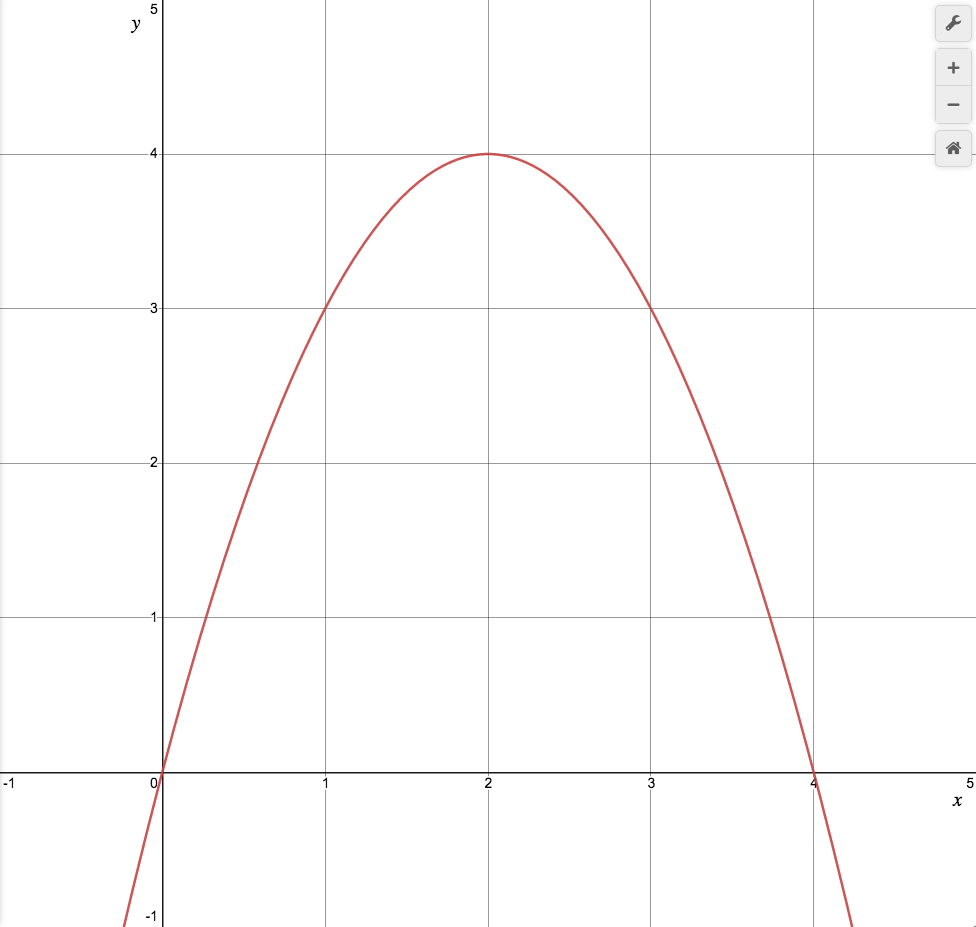
\includegraphics[scale=0.15]{\filePathGraphics/RQ12A_Graph.png}% Activate for quiz.
%\includegraphics[scale=0.8]{\filePathGraphics/RQ12A_Graph_Lower.pdf}% Activate for solutions.
\hspace{1in}
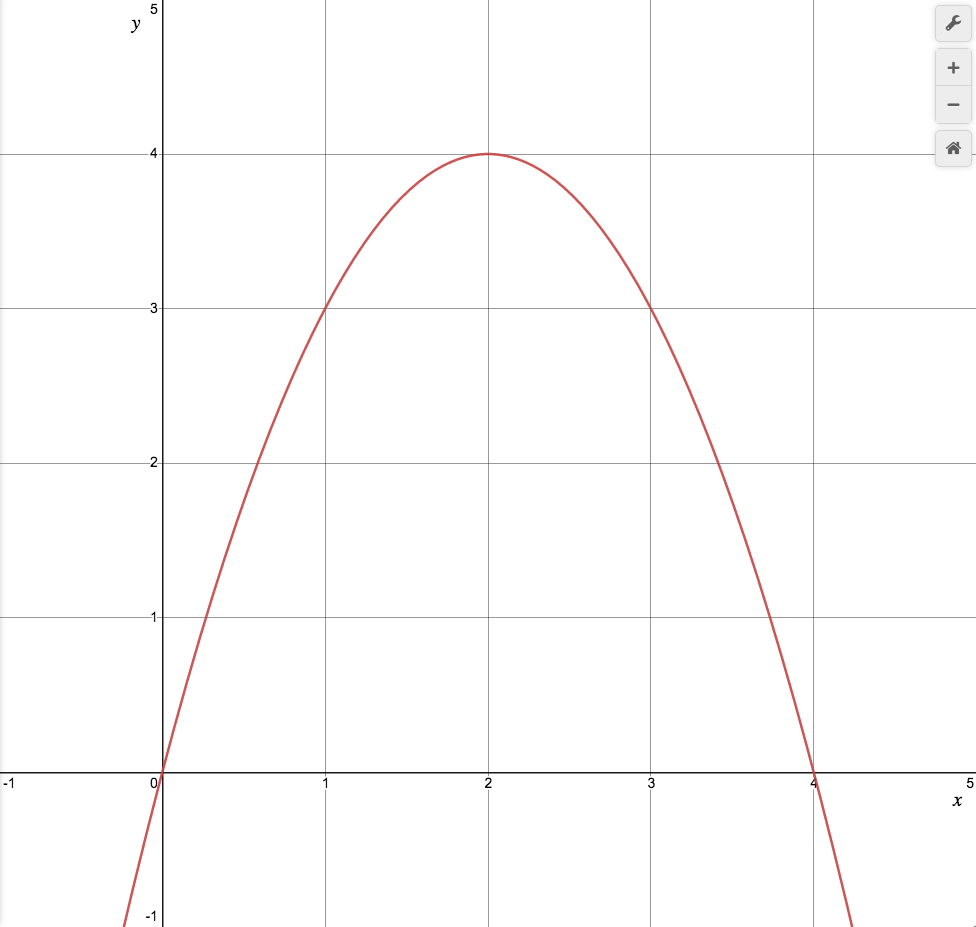
\includegraphics[scale=0.15]{\filePathGraphics/RQ12A_Graph.png}% Activate for quiz.
%\includegraphics[scale=0.8]{\filePathGraphics/RQ12A_Graph_Upper.pdf}% Activate for solutions.
\\
Lower sum ($L$)
\hspace{2in}
Upper sum ($U$)
\end{center}
\end{enumerate}

\spaceSolution{1in}{% Begin solution.
}% End solution.



\begin{enumerate}[resume,label=(\alph*)]
\item\label{itm : RQ12Ac} (1 pt) Find an antiderivative $F(x)$ of $f(x)$. Compute the difference $F(4) - F(0)$. Compare the result to the lower and upper sum you computed in part \ref{itm : RQ12Ab}.
\end{enumerate}

\spaceSolution{2in}{% Begin solution.
}% End solution.